%\textit{Introduce topic by talking about cells. Attention grabber, relate biophysics study to cancer reserach and many areas where we need to focus our research. Short and sweet, maybe 1 or 2 short paragraphs.}

	Neurodegenerative diseases, such as Alzheimer's or Huntinton's disease, are a leading cause of death in the United States \cite{eschbach2011cytoplasmic}. Scientists have yet to find a prevention or cure to these fatal diseases but suggests that motor protein failure directly contributes to cell degeneration. More specifically, defects in the motor protein dynein have been linked to neurodegeneration due to the cell's funtional dependence on dynein and its mechanical properties. However, dynein possesses a unique structure causing it to stochasitcally move around the cell and be unpredictable in nature. Thus, fully understanding the mechanisms of dynein can allow us to further understand causes of its failure. In this paper, we propose a model of dynein that uses Monte Carlo methods and a Brownian dynamics simulation to reproduce dynein's unique steping behavior. What follows is a brief introduction to the dynein motor protein, a review of the powerstroke model, and the framework for a computational simulation of the powerstroke, which we seek to replicate Yildiz's observation of correlated stepping \cite{Dewitt2012}.  

\section{Background}

\begin{figure}[H]
	\centering
	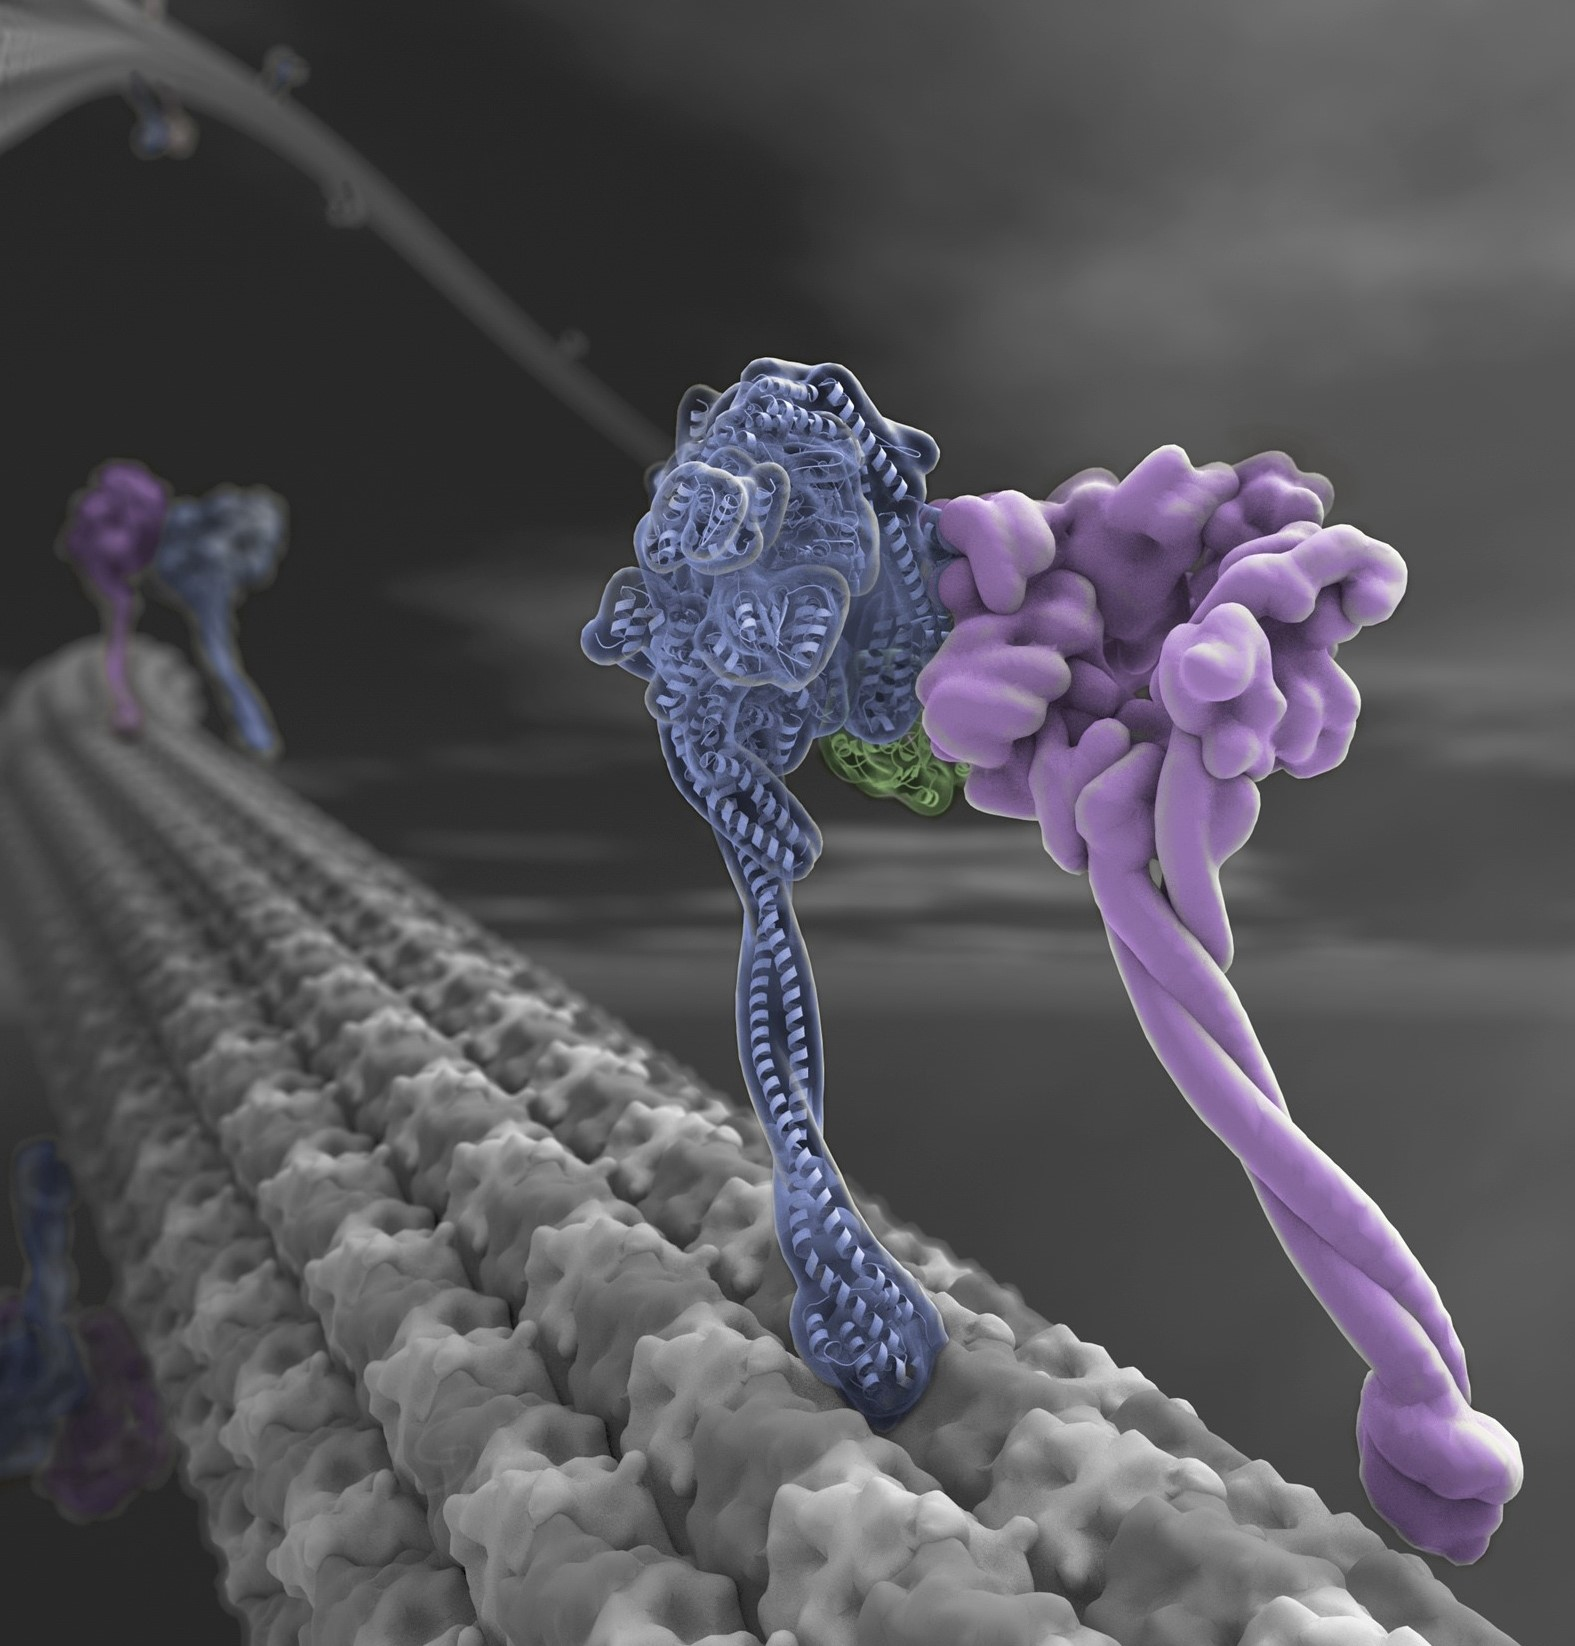
\includegraphics[width=0.3\columnwidth]{Figures/dynein_walking_art.jpg}
	\caption[Artist Rendition of Dynein]{\textbf{Artist Rendition of Dynein} walking along a microtubule in a cell. \cite{JohnsonArt}}
	\label{fig:ArtDynein}
\end{figure}

Cells are complicated. They have the ability to move, perfectly divide, and spatially organize themselves but are responsible for fatal diseases when these functions fail. Their functionality entirely depends on two-legged molecular proteins, named \textit{motor proteins}, that carry information along a microtubule track. These microtubules form the cytoskeleton in the cell and act as a walkway for the proteins (see Figure (\ref{fig:ArtDynein})). These motor proteins are myosin, kinesin, and dynein and are shown below in Figure (\ref{fig:Compare}). Because of kinesin and myosin's compact structure being close to the microtubule, their legs take turns alternating steps like a human and exhibit a uniform ``hand-over-hand" stepping pattern. On the other hand, dynein's structure involves two autonomous motors that cause inconsistent steps. As opposed to kinesin and myosin's uniform stepping, dynein exhibits an inchworm walk with one leg consistently ahead of the other, emulating a limping motion.

\begin{figure}[H]
	\centering
	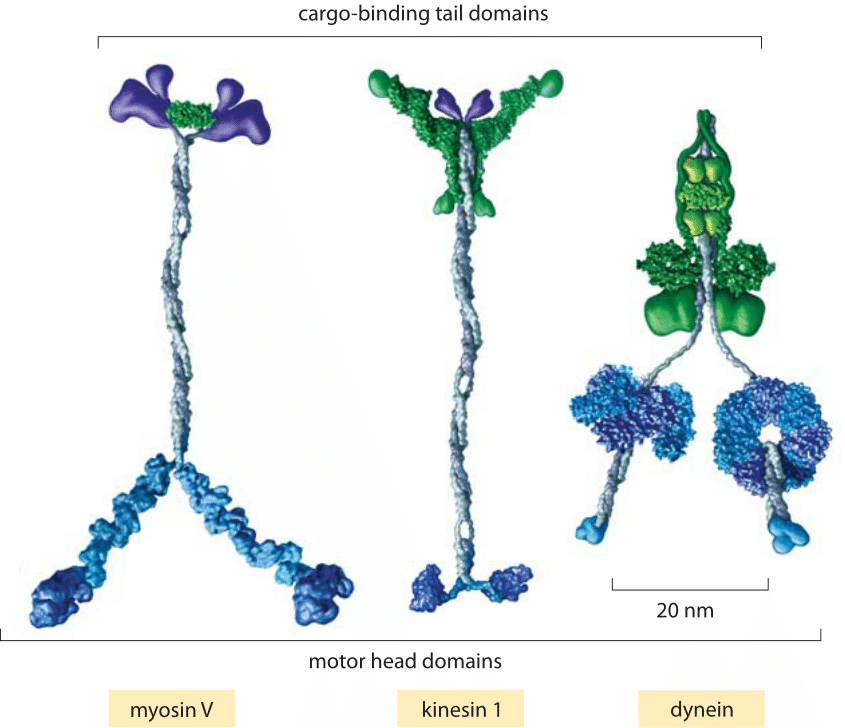
\includegraphics[width=0.4\columnwidth]{Figures/motor_comparison.png}
	\caption[Motor Proteins]{\textbf{Motor Proteins} Structure of myosin, kinesin, and dynein. \cite{JohnsonArt}}
	\label{fig:Compare}
\end{figure}

In addition to their structural differences, dynein walks towards the negative end of the microtubule while its motor protein siblings walk towards the positive end. Because microtubules are protein dimers constructed from negatively charged $\alpha$- and positively charged $\beta$-tubulins, the microtubule track is polarized depending on which tubulin dominates at the end points. In a eukaryotic cell, microtubules typically stem outwards from the cell's nucleus to the cell walls where the $\beta$ tubulin is exposed, generating a negative end at the nucleus and influencing dynein's directionality. Figure (\ref{fig:transport}) displays kinesin and dynein experiencing a charged attraction to the end points, while they share a cargo to deliver information during axonal transport. 

\begin{figure}[H]
	\centering
	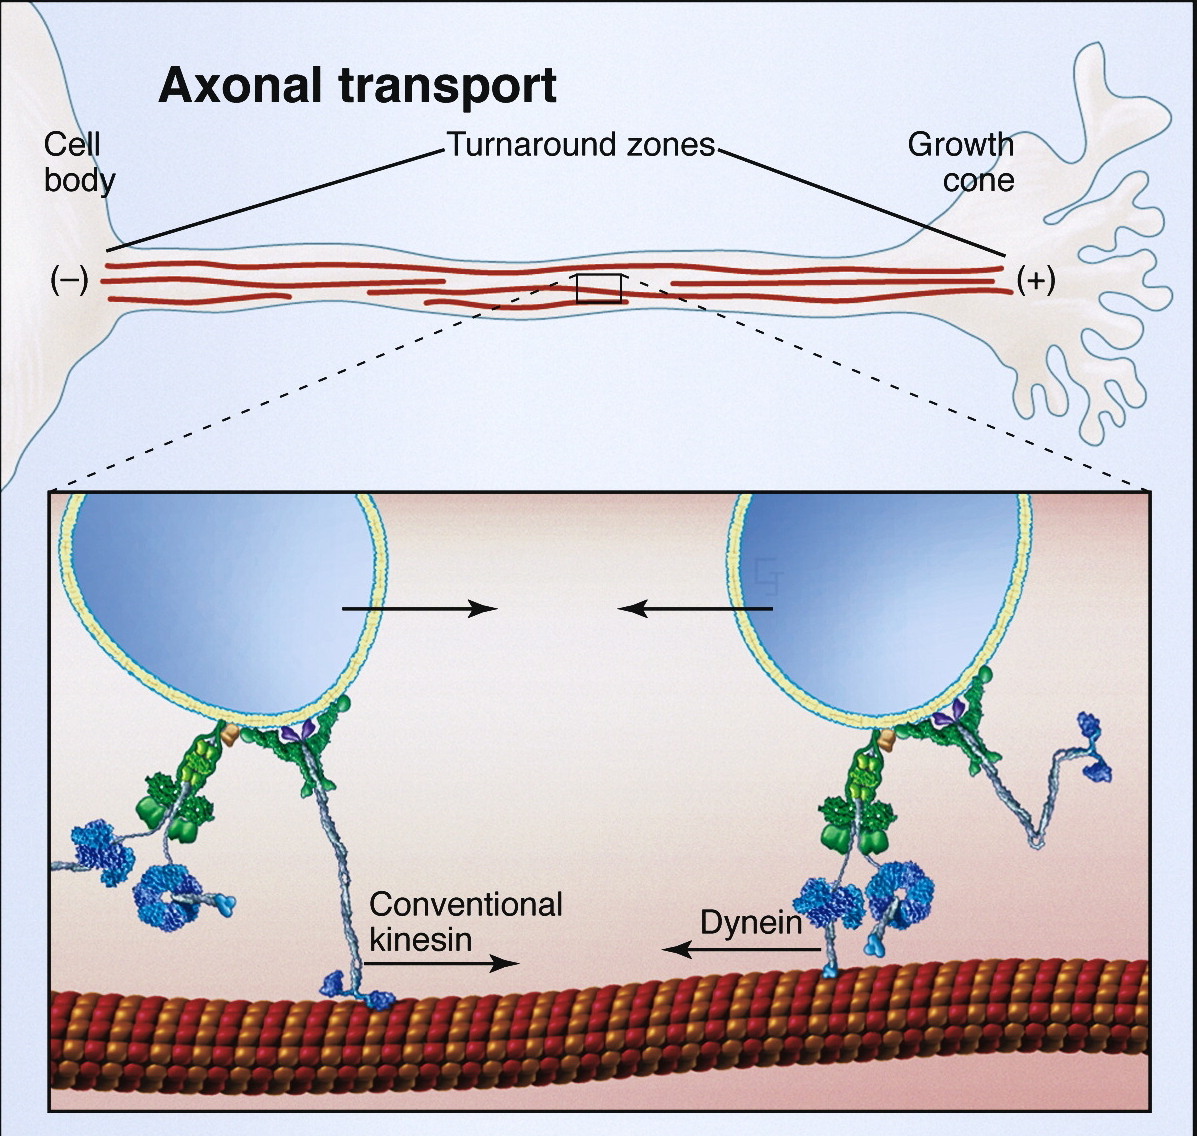
\includegraphics[width=0.6\columnwidth]{Figures/retrograde_transport.jpg}
	\caption[Charge Influenced Transport]{\textbf{Charge Influenced Transport}. Dynein and kinesin transporting cargo with information on the axon of a neuron cell for building the axon growth cone. They share cargo and take turns delivering each other to opposite ends of the cell. \cite{Vale2003molecular}}
	\label{fig:transport}
\end{figure}

These unique properties make dynein difficult to study when analyzing possible sources of molecular failure, but illustrates the importance of understanding its entire physical structure and the chemical interactions with ATP to produce motion.

\newpage
\section{Structure}
%\textit{In-detail background knowledge on structure of dynein. Talk about each domain and their roles. Binding domain, six AAA+ domains, tail, and cargo. Stalk and linker that attaches things together. How the structure is so much larger than that of kinesin. dynein has flexibility because of its linker and in order to compensate for its huge domains. }

Dynein's ``leg" is a complex protein assembly composed of linked amino acids subunits, called polypeptides, separated into three main domains. Figure (\ref{fig:structure}) displays these as the tail, the AAA+ rings (or motor), and the microtubule binding domain. The tail and the motor domains are connected by separate linkers, while the motor and the binding domains are connected by stalks. Both the linker and stalk measures greater than 20 nm in length, causing dynein to stand up to 50 nm high. 

%\begin{figure}[H]
%	\centering
%	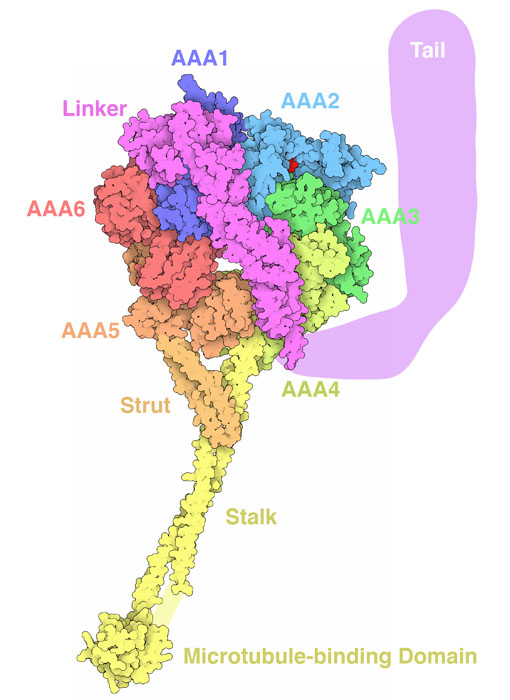
\includegraphics[width=0.6\columnwidth]{Figures/dynein_polypeptide.jpg}
%	\caption[Polypeptide Structure]{\textbf{Polypeptide Structure} \cite{GoodsellArt}}
%	\label{fig:polypeptide}
%\end{figure}

\begin{figure}[H]
	\centering
	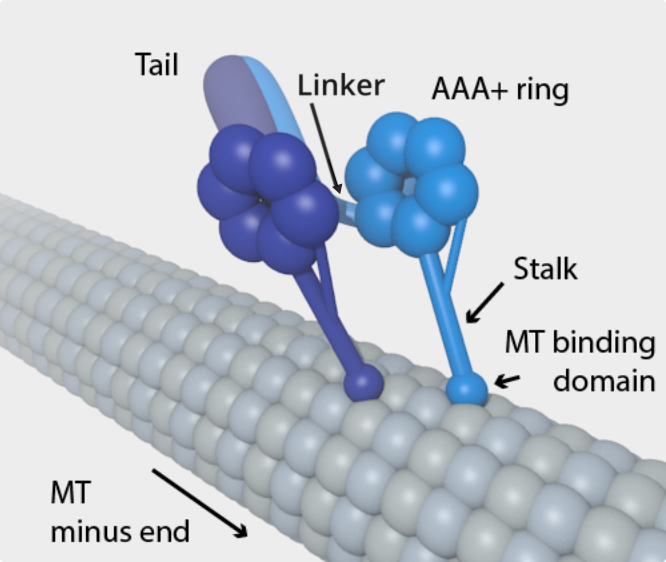
\includegraphics[width=0.6\columnwidth]{Figures/dynein_on_MT.png}
	\caption[Structure of Dynein]{\textbf{Structure of Dynein.} Illustration of cytoplasmic dynein's heavy chain subunits bounded to the microtubule. The AAA+ rings block the view of the linkers connecting them to the tail. For simplicity, this rendition depicts dynein’s structure as a domain-rod system. \cite{TheTrappistArt}}
	\label{fig:structure}
\end{figure}

Dynein's physical structure has been rigorously studied because of the pivotal role it plays in dynein's unpredictable stepping nature. Its inability to step uniformly is due to the large lengths between each major domain site, as the linker and stalk are 1.5x larger than the diameter of the AAA+ ring. In kinesin and myosin, the motor domains are much closer to the microtubule, causing a more controlled and consistent step due to their low center of mass. Despite dynein's large structure, it can still achieve processive stepping due to the interaction of adenosine triphosphate (ATP) with the AAA+ domains, which is why the AAA+ domains are referred to as the motor domains.





\section{Stepping}
%\textit{Biology and chemistry of stepping. What is actually causing it to step? ATP hydrolysis. Maybe short introduction on stepping and go more in detail in Power Stroke model. Say there are multiple theories and models of how dynein steps. Powerstroke, Winch, etc. Power stroke is most accepted. It can step on microtubule that is made up of tubulin dimers, $\alpha$ and $\beta$ tubulins. They are normally 8nm apart and so experimentalists believe dynein average step is always factor of 8nm. }

Dynein's ability to step is entirely ATP driven under the process of ATP hydrolysis. The ATP binds onto the motor domain and converts chemical energy into mechanical energy for dynein to transition between different conformational states (physicial arrangements) during a step. This process allows the binding domains to unbind and reattach at different locations on the microtubule and thus, permit varying step sizes. To measure dynein's step, an axis is defined on the microtubule.

The on-axis is defined parallel to the direction of forward stepping towards the negative end of the microtubule, while the off-axis is perpendicular, as shown in Figure (\ref{fig:axis}). Figure (\ref{fig:axis}) also displays the alternating helix structure of the $\alpha$- and $\beta$-tubulin dimers, in which act as the landing zones for dynein's binding domain.  

\begin{figure}[H]
	\centering
	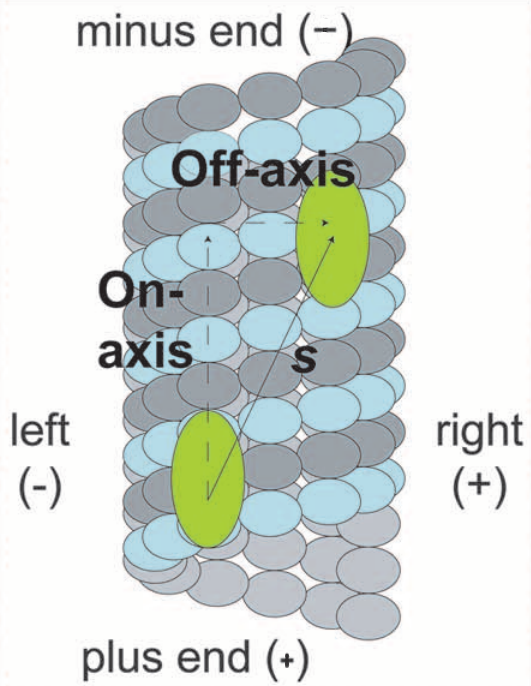
\includegraphics[width=0.3\columnwidth]{Figures/Onaxis.png}
	\caption[Stepping Axis]{\textbf{Stepping axis.} Birds-eye view of the microtubule with the green areas identifying the microtubule binding domains. For the on-axis, positive displacement is defined towards the minus end of the microtubule. Dark grey and light blue helix structure indicates $\alpha-$ and $\beta-$tubulin dimers, which are on average 8 nm apart in the on-axis. \cite{Dewitt2012} }
	\label{fig:axis}
\end{figure}

While ATP hydrolysis dictates the forward stepping during dynein's walk, the geometry of the domains is still a question for experimentalists. How exactly do the motor, tail, and linker achieve processive motion? Do the motor domains act as knees and stretch out for a step? Or do the knees stay bent, while the tail swings forward? Despite ongoing debates, researchers suggest the former and named this process the powerestroke model. 



\subsection{Powerstroke Model}
%\textit{Theorized model of stepping. Mechanochemical Cycle. Talk about ATP hydrolysis. Different conformational changes within a step. Look at linker and how it changes angles. Physically, it looks like it unbinds, stretches leg, then kicks forward, then diffuse back to MT.} 

The widely accepted powerstroke model was best exhibted within the mechanochemical cycle introduced by Cianfrocco et al. \cite{Cianfrocco2015mechanism}. A summary of the eight step cycle is shown below in Figure (\ref{fig:MechanochemicalCycle}).

\begin{figure}[H]
	\centering
	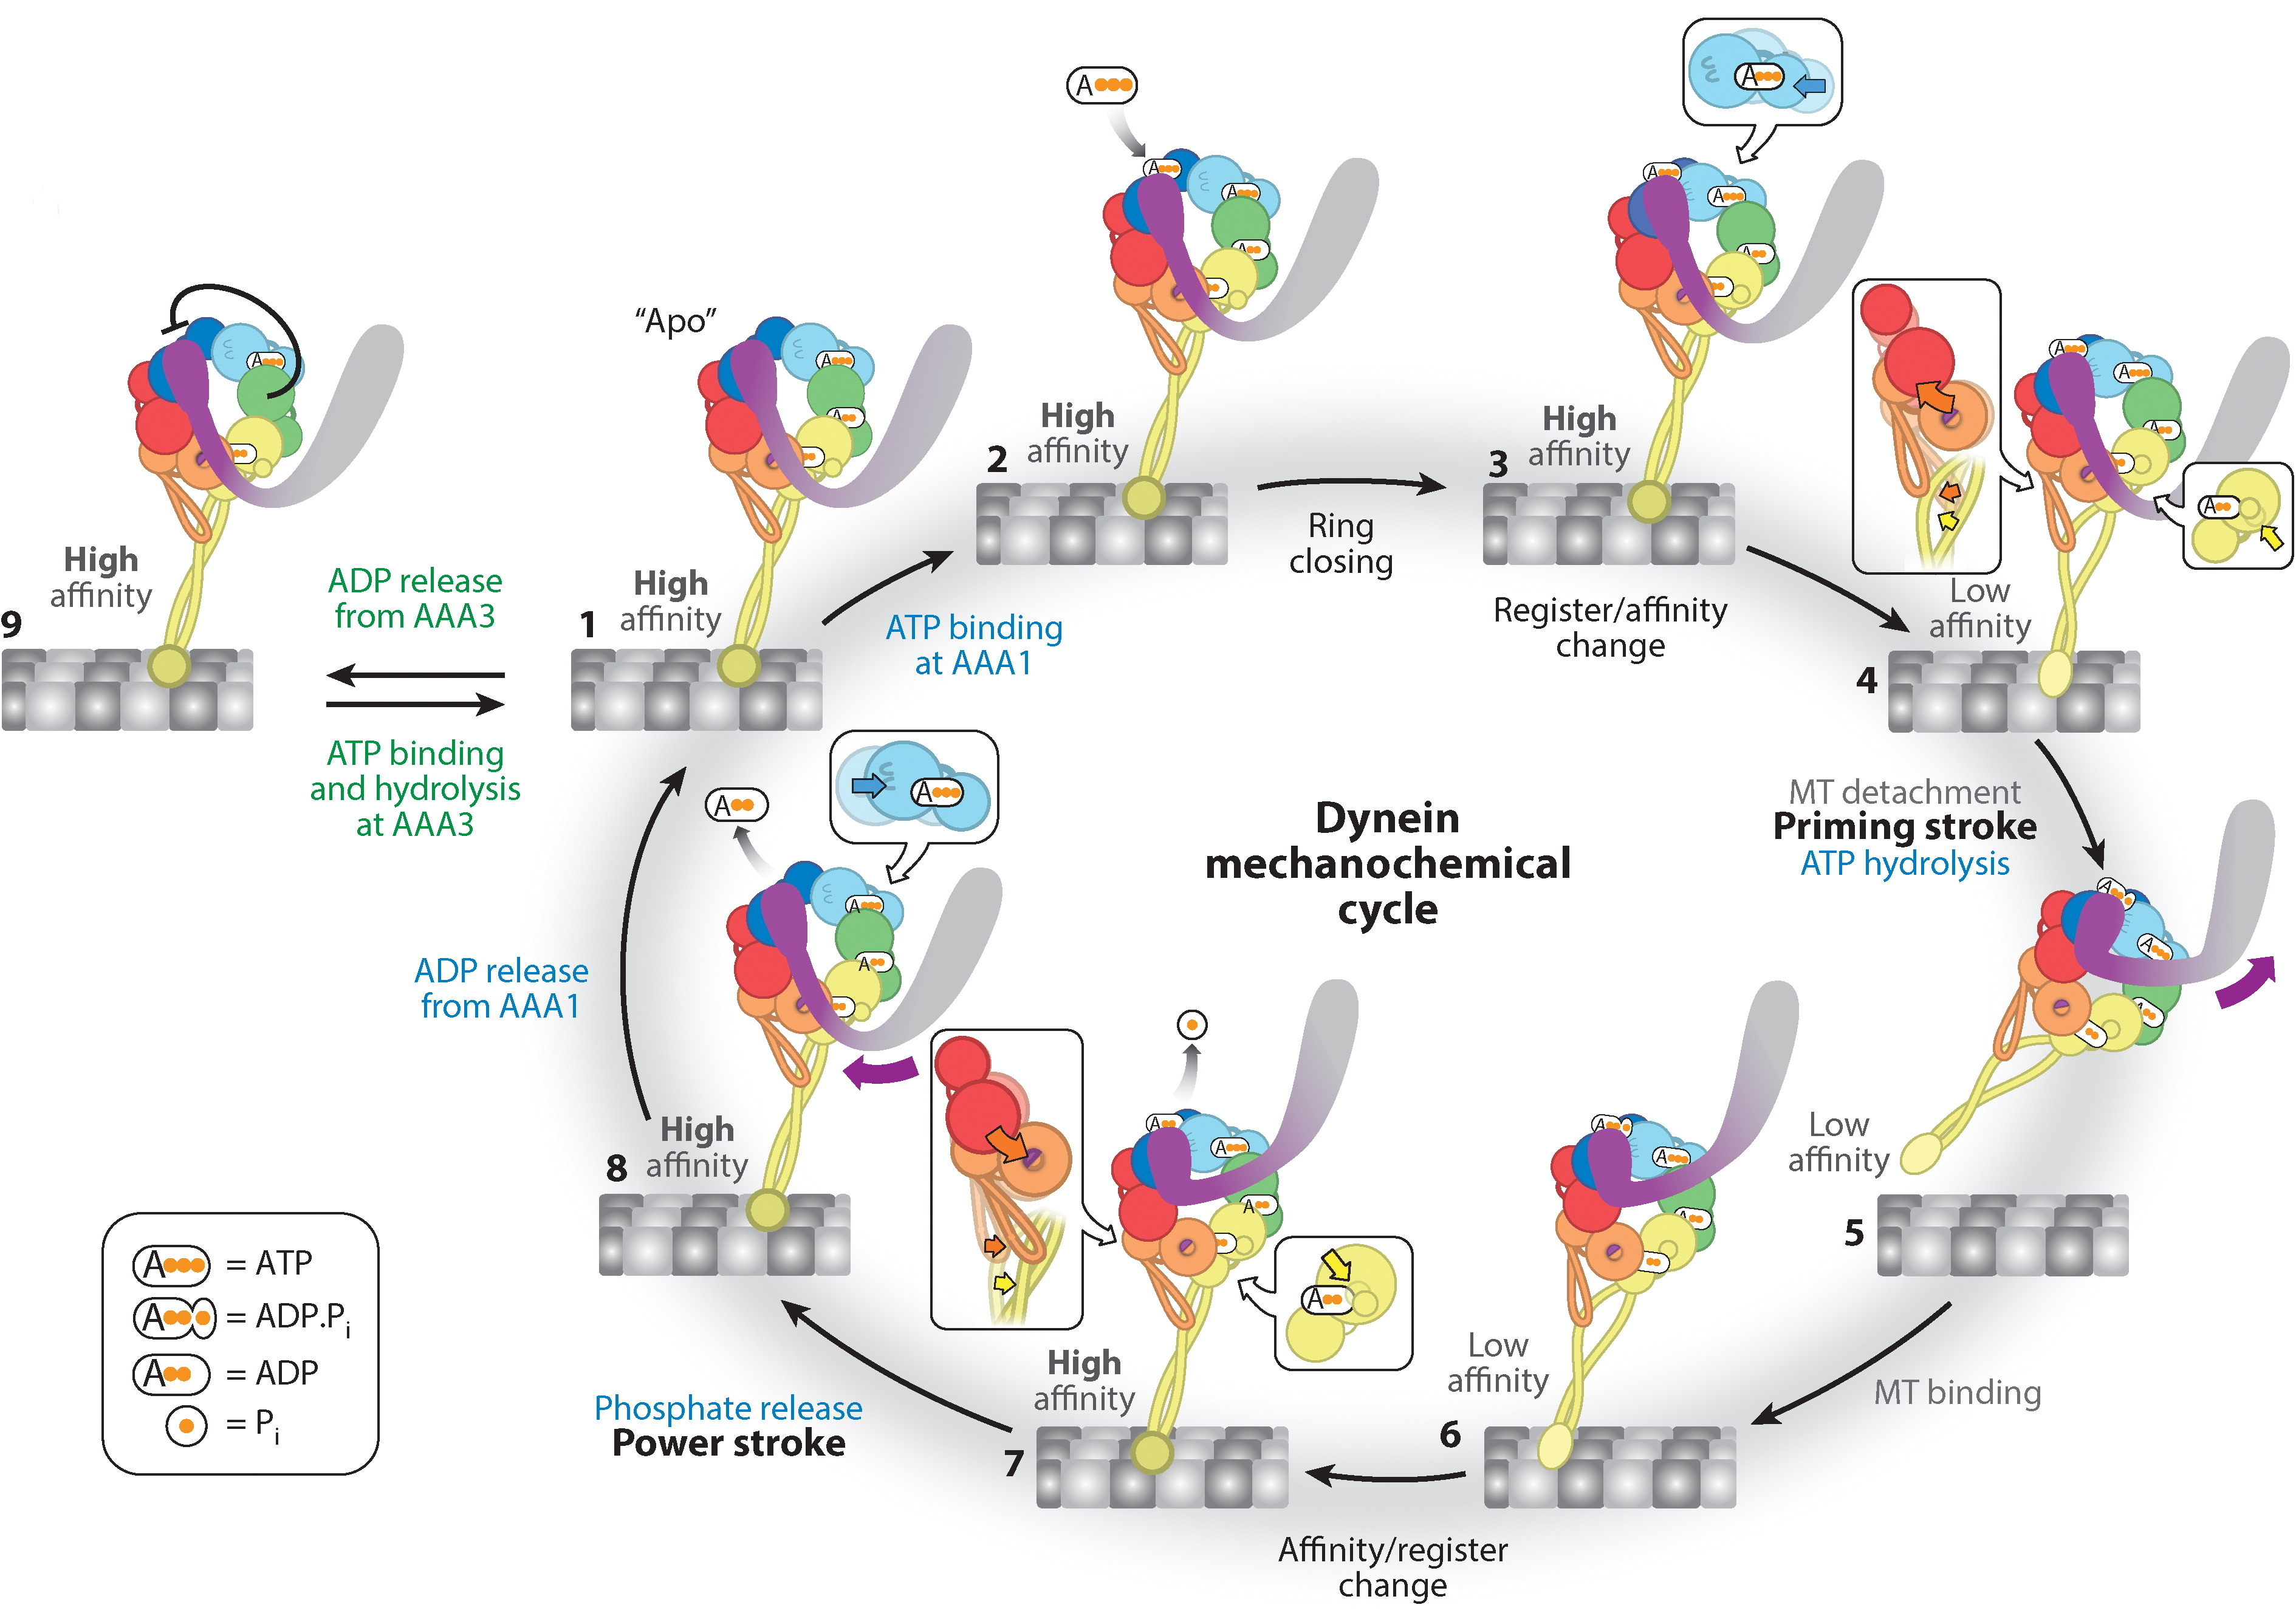
\includegraphics[width=1\columnwidth]{Figures/mechanochemical_cycle.jpeg}
	\caption[Mechanochemical Cycle]{\textbf{Mechanochemical Cycle.} The proposed series of conformational stages dynein undergoes during a step. The interaction of ATP with the motor domain is the main cause of the powerstroke, and high and low affinity indicated by the tightness of yellow polypeptides in the stalk. \cite{Cianfrocco2015mechanism}}
	\label{fig:MechanochemicalCycle}
\end{figure}

Here, affinity refers to the tendency and strength of the domain binding to the microtubule - high affinity being a secure attachment to the microtubule, while low affinity is more relaxed. The cycle utilizes the conformational transitions between high and low affinity to explain dynein's unbinding and rebinding process. This transition is governed by the addition of an ATP unit, which loosens the ``foot" from the MT (steps 3 to 4), stretches the linker (steps 5 to 6), and tightens the ``foot" back onto the MT (steps 6 to 7), pulling the whole protein forward. This key detail within the transition of stretching the linker distinguishes a ``pre-" and a ``post-" stroke state during the powerstroke model and can be analogous to bending a knee upwards and kicking the foot forwards to stretch the knee and take a step. A closer visualization of this transition between pre- and post-stroke states can be seen in Figure (\ref{fig:Powerstroke}), where the linker is highlighted in yellow.  

\begin{figure}[H]
	\centering
	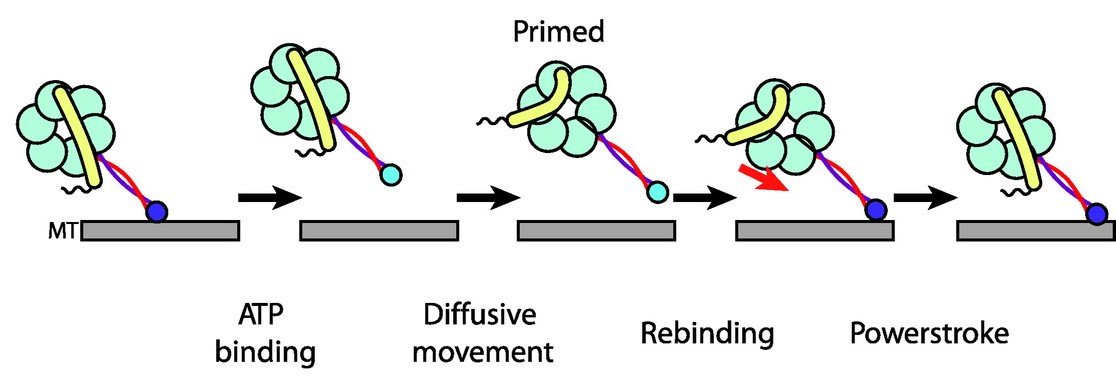
\includegraphics[width=1\columnwidth]{Figures/powerstroke.jpeg}
	\caption[Powerstroke]{\textbf{Powerstroke.} A more detailed visualization of the linker during the transition from pre- to post-stroke states. The linker is initially bent inwards during the pre-stroke state, then stretches backwards to extend the binding domain forward and land during the post-stroke state. \cite{Carter2010communication} }
	\label{fig:Powerstroke}
\end{figure}

Although the mechanochemical cycle provides a reasonable model for dynein's step and illustrates the motion between the domains, the model still generalizes the dependence on the configuration of the entire dynein (not just one motor) before the step and fails to analyze different geometric factors that can alter the conformations.

\section{Experimental Research on Dynein}

Experimental research investigates the correlations within dynein's step and how different parameters may affect the pattern. These consist of the angle dependency during the stretching of the linker, the effect of the initial domain distance before the step, the ATP concentration for hydrolysis, etc. However, due to dynein's small scale, experiment often disagrees with one another and differ depending on the various measuring techniques. 

%Although the mechanochemical cycle provides a reasonable model for dynein's step, the model fails to analyze the precise movements of each domain and how different configurations alter the conformational transitions. To what extent does the linker stretch when exhibiting the powerstroke and is it angle dependent? How does the separation between the two subunits of dynein affect the step length of the powerstroke? Consequently, these questions inspire experimentalists to measure dynein's step and study correlations between different parameters within a step.

\subsection{Measuring}
%\textit{How are experimentalists measuring dyneins stepping? Quantum dots on motor domains or quantum rod on tail, etc. }

Experimentalists measures dynein in various ways that utilizes electron microscopy and quantum measuring devices. Some attach quantum dots to dynein's motor domains, while others replace the tail with an artificial quantum rod. Despite the different procedures, all measuring techniques suffer from their inability to measure steps within $\sim 0.4$ nm of where the binding domain lifted off. This causes short step lengths, where the binding domain quickly rebinds after unbinding, to be undetectable. The various measuring procedures and experimental limitations leads to different results and unique findings when observing different variables. In this paper, we focus on the unique observation by Yildiz \textit{et al.} of a stepping correlation between the initial interhead separation and step length because of the results contradicting previously accepted theories of independent stepping. 


\subsection{Yildiz's Stepping Correlation}
%\textit{Purpose of my research. Trying to make model and fit to Yildiz analysis of dynein having interstep correlation. Dependency between step length and initial inter head separation.}

Due to dynein's large size and stochastic nature, dynein's step was previously hypothesized to be independent from the initial conformational before the step. However, in 2012, Yildiz \textit{et al.} observed a correlation between the initial on-axis separation and the step length, indicating a dependence on the interhead separation \cite{Dewitt2012}. This discovery challenged established views on dynein's stepping processivity and pose the question of whether there exists interhead coordination between the motor domains when stepping. Figure (\ref{fig:YildizCorrelation}) below displays this correlation with a linear regression, where an existing non-zero slope indicates a dependence between the step and the initial on-axis separation.

\begin{figure}[H]
	\centering
	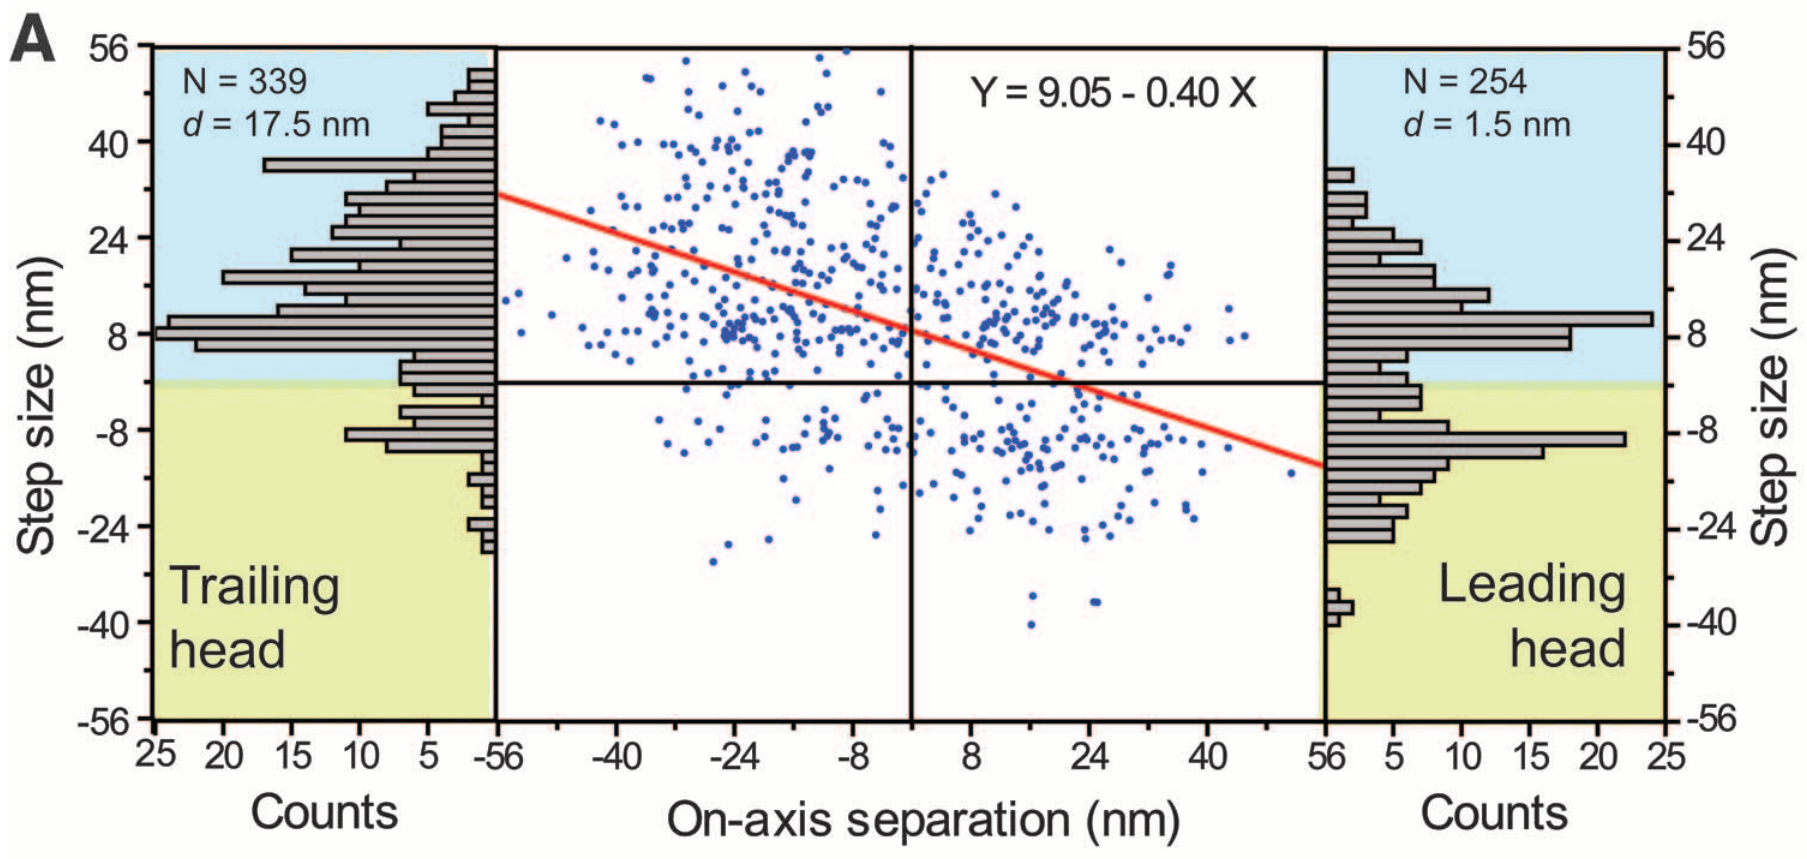
\includegraphics[width=1\columnwidth]{Figures/Yildiz_stepping.png}
	\caption[Stepping Correlation]{\textbf{Stepping Correlation.} A scatter plot of step sizes vs. on-axis separation which hints at a functional dependency between the step  length and the initial distance between the binding domains. The 1D histogram for the trailing head on the left records the step lengths for the negative on-axis separation, while the histogram for the leading head does the same for positive on-axis separation. \cite{Dewitt2012} }
	\label{fig:YildizCorrelation}
\end{figure}

This correlation implies a connection between the physical state of dynein and its stepping behavior, inferring that dynein's step is not only ATP dependent. Because of the limited sample size from experiment producing a unique correlation, observations like Yildiz's can massively benefit from accurate computational models that can simulate dynein's stepping under realistic circumstances.




\section{Motivation}
%\textit{Briefly write about the importance of dynein, how dynein is researched when studying neurological diseases, dynein stepping is understudied compared to other motor proteins, hard to model dynein because of random walking, there are almost no computational models of dynein that uses molecular dynamics, modelling dyenin can give us better understanding of why it moves the way it does, specific motivation for model: new research found that there is interhead coordination when stepping so maybe we can use that to base our model off of.}

We want to further investigate Yildiz's unique stepping correlation by creating a compuational simulation of dynein and analyze the specific conditions that are required to replicate their results. Currently, other simulations that model dynein's step exist, but all of them are used to investigate the ATP hydrolysis mechanism during the mechanochemical cycle. These simulations suffer from numerous assumptions made about the physical aspects of dynein's step. (\textit{Should reference a simulation here}) Some assume that dynein can step only in increments of 8nm or that the rebinding process is constrained to a certain time frame. These limitations make it impossible for their models to replicate mechanical phenomenon observed in dynein's stepping, such as Yildiz's correlation from above.

To bridge this gap, Roundy \textit{et al.} constructed a physical model of dynein that explores the molecular interactions between the domains of dynein and its aqueous environment. Instead of making assumptions about the physical mechanics of the step, Roundy's model neglects the chemistry of the ATP exchange and assumes the energy transfer from ATP is incorporated within the binding processes. Researchers John Waczak and Elliott Capek successfully incorporated this model under an angle-dependent Brownian dynamics simulation, where each domain experienced Brownian motion to mimic stochastic movement \cite{Capek2017, }. They were able to track dynein's precise movement along a walk and compare their stepping results to experiment. However, they also discovered that dynein spends less than 5\% of its total stepping time in the low affinity state where the dynein exhibits the actual stepping motion ($<1$ ms unbound while $>20$ ms bound). Because of this, their simulation suffered from immense computation time and lacked the ability to optimize model parameters for a better fit to experiment. For this work, we will use their simulation as a foundation but replace the dynamical bounded state with a Monte Carlo algorithm. This allows us to only simulate the stepping motion, as the Monte Carlo will initially test equilibrium configurations before the step. This new method will drastically shorten computation time and generate larger ensembles of statistics. We intend to use this model to reproduce experimental measures and help verify existing understandings concerning the properties of dynein’s stepping mechanism. More specifically, we want reproduce Yildiz's unique findings and investigate the stepping dependence on the interhead separation. 



%\textit{THIS IS STRAIGHT FROM PROPOSAL, NEED TO FIX THIS AND ADJUST SO THAT MORE DYNEIN DETAILS GOES INTO CHAPTER 2}
%
%In a eukaryotic cell, dynein is one of the three motor proteins that are responsible for the cell’s ability to move, divide, and spatially organize itself. Similar to the more researched kinesin, dynein conveys cargo along the microtubule track by using ATP to power its two binding domains (its “feet”). However, its walking-like movements along the track are very unpredictable and can vary in terms of distance and direction. Dynein’s two feet can also act independently from each other causing much more erratic and stochastic steps. However, despite dynein’s stochastic nature, dynein is still able to achieve processive motion due to the functions of its structure. Structurally, dynein is composed of two motor heavy chain subunits of linked amino acids, called polypeptides, each which are separated into domains. These domains are the tail domain, the linker domain, the six AAA+ domains, and the microtubule binding domains (See Figure 1). The AAA+ domains are responsible for ATP hydrolysis, in which converts chemical energy stored in ATP into mechanical work causing dynein’s motility. 
%
%Because dynein’s stepping is unpredictable in nature, its stepping mechanism has not been intensely studied as compared to its structure. Questions regarding the electrostatic interactions with the microtubule, ring stacking, discrete microtubule binding sites, or elasticity of the stalk are yet to be answered. A known and supported model to describe dynein’s motion is the powerstroke model, where ATP binding to an AAA+ domain triggers conformational changes that lowers the affinity of the binding domain for the microtubule, causing it to unbind and take a step . While the powerstroke model and other theorized stepping models exists, there are no such studies which use molecular dynamics to verify if these theorized mechanisms are feasible for the dynein motor to produce. There are studies that incorporate a computational model of dynein, but many use chemical rate transitions and assume independence of steps without simulating the precise protein dynamics within its step.
%
%To bridge this gap, we propose a coarse-grained model of dynein that assumes a particle-rod structure for its various domains and uses Brownian motion to simulate the model’s behavior in physically realistic drag and diffusion conditions, while efficiently collecting a wide ensemble of statistics using Monte Carlo methods. We chose to use Brownian inspired motion to simulate dynein’s molecular dynamics in order to replicate dynein’s stochastic behavior under realistic conditions and produce its unpredictable stepping patterns observed from experiment. We call this process Brownian dynamics, as it replaces interactions the domains have with solvent molecules with a stochastic force and allows us to simulate large time scales compared to other molecular dynamics simulation. Likewise, Monte Carlo methods will allow us to visualize dynein as a system and associate its possible configurations as states. With our simulation following these methods, we can generate an ensemble of statistics and compare measured quantities with experiment. We intend to use this model to reproduce experimental measures and help verify existing understandings concerning the properties of dynein’s stepping mechanism. One of which being a question regarding dynein’s inter-step correlation. 

